\chapter{Materials and Methods} \label{ch:Materials and Methods}

\section{Cell Culture} \label{sec:Cell Culture}
\subsection{Cell Culture Conditions} \label{subsec:Cell Culture Conditions}
All cell lines listed in Table \ref{tab:Cell Lines Table} were cultured in cell culture flasks (Corning) at 37°C in a 5\% \ch{CO2} atmosphere. All cell lines with the exception of BEAS-2B were maintained in complete Dulbecco’s Modified Eagle’s Medium (DMEM; Sigma-Aldrich) supplemented with 10\% Foetal Bovine Serum (FBS, Sigma-Aldrich), 1\% L-Glutamine (Sigma-Aldrich) and 1\% penicillin and streptomycin mixture (TermoFisher). BEAS-2B cell line was cultured in LHC basal medium (TermoFisher), supplemented with 10\% FBS (Sigma-Aldrich), 1\% L-Glutamine (Sigma-Aldrich) and 1\% penicillin and streptomycin mixture (TermoFisher).

\begin{table}
\centering
\begin{tabular}{|l|l|l|ll}
\cline{1-3}
Cell Line & Description & Source & &  \\ \cline{1-3}
VERO & monkey   kidney epithelial cells & \\ \cline{1-2}
A549 & human alveolar epithelial cancer cells & & &  \\ \cline{1-2}
HEK293T & human embryonic kidney cells & & &  \\ \cline{1-2}
MDBK & Madin-Darby bovine kidney cells & & &  \\ \cline{1-2}
BT & bovine turbinate epithelial cells & & &  \\ \cline{1-2}
HeLa & human uterine epithelial cancer cells &
  \multirow{-6}{*}{\begin{tabular}[c]{@{}l@{}}The Pirbright Institute's \\ Central Services Unit \\ (CSU)\end{tabular}} &
   &
   \\ \cline{1-3}
BEAS-2B & human bronchial epithelial cells & ATCC & &  \\ \cline{1-3}
\end{tabular}
\caption[Cell lines used in this study.]{\textbf{Cell lines used in this study.}}
\label{tab:Cell Lines Table}
\end{table}




\subsection{Passaging and Seeding Cells} \label{subsec:Passaging and Seeding Cells}
All cell lines were grown until ~80\% confluent, at which point the growth media was removed and cells were washed with sterile Phosphate Buffered Saline (PBS). Cells were detached from the flasks using Trypsin/EDTA solution (Life Technologies). After complete detachment, cells were diluted in complete media and 5\% of the cells were transferred to a new flask for further passaging. The reminding cells were used for seeding for experiments.




\subsection{Transfecting Cells} \label{subsec:Transfecting Cells}
Plasmids were transfected to well-adhered cells (>6 hours post seeding) using TransIT-X2 (Geneflow). Plasmid DNA was diluted in Opti-MEM (ThermoFisher), TransIT-X2 was added in 1:2 ratio (\(\mu\)g of DNA to \(\mu\)L of TransIT-X2), vortexed and then incubated at room temperature for 40 minutes. The transfection mix was added dropwise to cells and incubated at 37ºC and 5\% \ch{CO2} for the required times to allow protein expression.




\subsection{Treatment with the Activators of Innate Immune System} \label{subsec:Treatment with the Activators of Innate Immune System}
Several known activators of the innate immune system were used for cellular treatment (see Table \ref{tab:Activators of the Innate Immune System Table}). These were human and bovine interferon-alpha and gamma (IFN), \textit{E. Coli} lipopolysaccharide (LPS) and polyinosinic:polycytidylic acid (poly I:C). 2 \(\mu\)g of poly I:C was transfected as described in Section \ref{subsec:Transfecting Cells} and incubated for 24 hours. Concentrations used for bovine IFN\(\alpha\) were 0.5 and 5 ng/mL with an incubations of either 3, 6 or 24 hours. Human IFN\(\alpha\) was used in the concentration of 1000 units per mL, with the incubation time of 6 or 24 hours. Human IFN\(\gamma\) was used in concentrations of 500, 1000, and 2000 units per mL for a duration of 6 hours. LPS was used in a concentration of 5 and 5000 \(\mu\)g/mL for human cell lines and concentrations of 0.5, 1, 2.5, 5, and 10 for the bovine cell lines, for a duration of 6 hours.
 
\begin{table}
\centering
\begin{tabular}{ccc}
\hline
\textbf{Name} & \textbf{Provider}    & \textbf{Product Number} \\ \hline
Human IFN\(\alpha\)    & Sigma-Aldrich UK     & SRP4596                 \\ \hline
Bovine IFN\(\alpha\)   & Bio-Techne Ltd.      & RP0008B-025             \\ \hline
Human IFN\(\gamma\)    & PeproTech, Inc.      & 300-02                  \\ \hline
Bovine IFN\(\gamma\)   & Cambridge Bioscience & 2300-BG-025             \\ \hline
LPS           & Sigma-Aldrich UK     & L4391-1MG               \\ \hline
Poly I:C      & Sigma-Aldrich UK     & P1530-25MG              \\ \hline
\end{tabular}
\caption[Activators of the Innate Immune System.]{\textbf{Activators of the Innate Immune System.}}
\label{tab:Activators of the Innate Immune System Table}
\end{table}




\section{Virus Work} \label{sec:Virus Work}
\subsection{Virus Propagation and Production} \label{subsec:Virus Propagation and Production}
Viruses (outlined in Table \ref{tab:Outline of Viruses Used table}) were propagated in the VERO cell line. 70\% confluent T175 cell culture flask was incubated with 0.01 multiplicity of infection (MOI) concentration of virus of choice diluted in serum-free cell culture medium for 2 hours. Afterwards, the virus-containing media was washed away with PBS and cells were incubated in 2\% serum-containing growth media for 72 hours. After, cells were scraped into the media and the viral particles were liberated from cytoplasm by sonication. This was done at 70\% amplitude and 1 second long on and off pulses. Cell debris was separated by centrifugation at 2900 g for 30 minutes at 4°C. The supernatant was either snap-frozen in a dry ice ethanol mixture and stored at -80°C as crude extracted virus or was further purified. Further ultracentrifugation purification was conducted to ensure that all cytokines, chemokines, and other stimulants are removed from the viral stock. Crude extracted supernatants were mixed with \ch{MgSO4} (Sigma), 50\% (w/v) polyethylene glycol (PEG) 6000 (Sigma) in NT buffer (100mM \ch{MgSO4}, 150 mM \ch{NaCl} (Sigma), 1mM EDTA (Invitrogen), 50 mM Tris-\ch{HCl} (Sigma), pH 7.5) and serum-free DMEM to a final concentration of 100 mM, 10\% and 2.3\% (v/v) respectively. The solution was thoroughly mixed with a magnetic stirrer at 4°C for 90  minutes to precipitate the viral particles. Afterwards, the particles were pelleted by centrifugation at 2900 g for 20 minutes at 4°C and resuspended in 700 \(\mu\)L 4°C NT buffer. Finally, viral particles were separated and concentrated by ultracentrifugation at 32,000 rpm at 4°C for 1.5 hours in the SW-32 rotor on a discontinuous sucrose gradient. The gradient was prepared by sequential layering and freezing at -80°C 60\%, 45\%, and 30\% sucrose (Sigma) in NT buffer, placed in Ultra-Clear 14x95 mm centrifuge tubes (Beckman Coulter UK Ltd). The outcome was two viral bands (at 30-45\% and 45-60\% interface) which were both collected and snap-frozen in a dry ice ethanol mixture and stored at -80°C.

\begin{table}
\centering
\begin{tabular}{ccccc}
\hline
{\textbf{Virus name}} &
  {\textbf{Species}} &
  { \textbf{Strain}} &
  { \textbf{Modification}} &
  { \textbf{Source}} \\ \hline
hRSV      & Human  & A2     & WT   &  \\ \cline{1-4}
hRSV-GFP  & Human  & A2     & GFP  &  \\ \cline{1-4}
bRSV      & Bovine & A51908 & WT   &  \\ \cline{1-4}
BRSV-GFP  & Bovine & A51908 & GFP  &  \\ \cline{1-4}
bRSV \(\Delta\)SH  & Bovine & A51908 & \(\Delta\)SH  &  \\ \cline{1-4}
bRSV \(\Delta\)NS1 & Bovine & A51908 & \(\Delta\)NS1 &  \\ \cline{1-4}
bRSV \(\Delta\)NS2 & Bovine & A51908 & \(\Delta\)NS2 &  \\ \cline{1-4}
bRSV \(\Delta\)NS1/2 &
  Bovine &
  A51908 &
  \(\Delta\)NS1 \& \(\Delta\)NS2 &
  \multirow{-8}{*}{The Pirbright Institute} \\ \hline
\end{tabular}
\caption[Outline of Viruses Used.]{\textbf{Outline of Viruses Used.}}
\label{tab:Outline of Viruses Used table}
\end{table}




\subsection{Virus Quantification by TCID50 Assay} \label{subsec:Virus Quantification by TCID50 Assay}
Crude or ultra-purified samples from Section ref{Virus Propagation and Production} were thawed at room temberature and serialy diluted in 0\% FBS DMEM in 1:10 ratios in quadruplicates with final volume of 50 \(\mu\)L. A TC75 cell cuture flask with 100\% confluent permissive cell line of choise (preferably one that will be used for subsequent experiments) was trypsinised and diluted in 100 mL of 2\% FBS DMEM and 100 \(\mu\)L of it was dispensed per titration well. Plates were left to incubate at 37°C in a 5\% \ch{CO2} atmosphere for 4 days, after which they were analysed for the presence of cytopathic effects. This data was used to calculate the multiplicity of infection.




\subsection{Viral Infections, UV-Inactivation and Ruxolitinib Treatment} \label{subsec:Viral Infections, UV-Inactivation and Ruxolitinib Treatment}
Crude or ultra-purified samples from Section ref{Virus Propagation and Production} were thawed at room temberature. If the experimental procedure required UV-inactivation, the viral extract was placed in circular plastic dish, transfered to the UV cross-linker (COMPANY), and irradiated without the lid for 60 seconds at the power of WHATEVER. Cells at the confluency of 80\% had their media removed and were washed with PBS. Afterwards, the virus diluted at the desired MOI in serum-free cell culture media was added and samples were incubated at 37°C in a 5\% \ch{CO2} atmosphere for 2 hours. Afterwards, the inoculum was removed and replaced with 2\% serum cell culture medium and left to incubate at 37°C in a 5\% \ch{CO2} atmosphere. If the experimental procedure required the presence of ruxolitinib, it was mixed-in with the culture medium at 5 nM and cells were left to incubate at 37°C in a 5\% \ch{CO2} atmosphere until the end point of the experiment.




\subsection{Viral Growth Curves} \label{subsec:Viral Growth Curves}
Cells infected as described in Section \ref{subsec:Viral Infections, UV-Inactivation and Ruxolitinib Treatment} were collected as a supernatant and cellular fraction at time intervals of 24, 48, 72, 96, 120, 144, and 168 hours post-infection, snap frozen in dry ice ethanol mixture, and later tittered as described in Section \ref{subsec:Virus Quantification by TCID50 Assay}.




\section{Quantitative Real Time/Reverse Transcription PCR} \label{sec:Quantitative Real Time/Reverse Transcription PCR}
\subsection{RNA Extraction and cDNA Synthesis} \label{subsec:RNA Extraction and cDNA Synthesis}
Initially, cells were washed using phosphate-buffered saline (PBS; 137 mM \ch{NaCl}, 10 mM phosphate, 2.7 mM \ch{KCl}, pH 7.4) after which RNA was extracted using an RNeasy Mini Kit (Qiagen). The concentration and purity of samples were assessed using the NanoDrop One spectrophotometer (Thermo Fisher). Complementary DNA (cDNA) was synthesised using Moloney Murine Leukaemia Virus Reverse Transcriptase (MMLV RT; Promega). Firstly, RNA was mixed with oligo dT primers (Sigma-Aldrich) at a 2:1 ratio and the resulting mixture was topped up with nuclease-free \ch{H2O} to a final volume of 13 \(\mu\)L. Denaturation, which removes any secondary structures in the samples was done by incubation at 70°C for 5 minutes, followed by a step of rapid primer annealing by incubating the samples in icy water for 2 minutes. 12 \(\mu\)L of reaction master mix consisting of 5 \(\mu\)L 10 mM dNTPs, 5 \(\mu\)L MMLV RT Buffer, 1 \(\mu\)L of RNAse inhibitor and 1 \(\mu\)L of MMLV reverse transcriptase (Promega) was then added. Samples were then incubated at 42°C for 1 hour, after which they were diluted 1:4 using nuclease-free \ch{H2O}. As a control for DNA contamination evaluation, there was always at least one sample in which the MMLV RT was substituted with \ch{H2O}.




\subsection{Quantitative PCR} \label{subsec:Quantitative PCR}
RNA transcripts of interest were quantified using quantitative polymerase chain reaction (qPCR). Luna Universal qPCR Master Mix and Luna Universal Probe qPCR Master Mix (New England Biolabs) were used for SYBR-based and TaqMan-based qPCR, respectively. For SYBR-based method, 10 \(\mu\)L of Master Mix was mixed with template cDNA, 1 \(\mu\)L of primer set, and topped up to 20 \(\mu\)L by nuclease-free water. Probe-based sample preparation only differs in using 2 \(\mu\)L of primer/probe mix instead of the above mentioned 1 \(\mu\)L. Samples were run on the QuantStudio 3 Real-Time PCR System (Thermo Fisher) on a MicroAmp Fast Optical 96-Well reaction plates (Fisher Scientific), sealed with MicroAmp Adhesive qPCR plate seal (Fisher Scientific). The temperature of the metal cover on the top was set to 105°C to prevent evaporation, and plates were run on a standard thermal cycling mode as depicted in Table \ref{tab:qPCR Cycling Conditions table}. The temperature changes between different stages were set to 1.6°C/s. During the extension step of the PCR stage, signal acquisition took place. For TaqMan-based qPCR only hold and PCR stages were run, whereas for SYBR-based qPCR the quality control step of melt curves acquisition was also conducted. During the transition from the annealing step of melt curve stage to the final step, the temperature increase was 0.1°C/s, with a continual signal acquisition.

\begin{table}
\centering
\begin{tabular}{lllllll}
\hline
Stage        & SYBR & TaqMan & Step                 & Temperature & Time & Cycle \\ \hline
Hold         & Yes  & Yes    & Annealing            & 50°C        & 2'   & 1     \\ \hline
Hold         & Yes  & Yes    & Initial Denaturation & 95°C        & 10'  & 1     \\ \hline
PCR          & Yes  & Yes    & Denaturation         & 95°C        & 15'' & 40    \\ \hline
PCR          & Yes  & Yes    & Extension            & 60°C        & 60'  & 40    \\ \hline
Melt   Curve & Yes  & No     & Denaturation         & 95°C        & 15'' & 1     \\ \hline
Melt Curve   & Yes  & No     & Annealing            & 60°C        & 60'' & 1     \\ \hline
Melt   Curve & Yes  & No     & Dissociation         & 95°C        & 15'' & 1     \\ \hline
\end{tabular}
\caption[qPCR Cycling Conditions.]{\textbf{qPCR Cycling Conditions.}}
\label{tab:qPCR Cycling Conditions table}
\end{table}




\subsection{Primer Design and Assay Setup} \label{subsec:Primer Design and Assay Setup}
To amplify specific regions of genes of interest, commercial forward-reverse primer with fluorescent probe were bought where available (see Table \ref{tab:Commercial qPCR Primers Table}). However, there were no available primers for amplification of bovine \textit{IFIT} genes. For this reason, these primers were designed \textit{in silico}. Using coding DNA sequences obtained from ENSEMBL database (\cite{Cunningham2022Ensembl2022}) and the PrimerQuest software (Integrated DNA Technologies) with its default parameters (50 mM of monovalent salt, 3 mM of bivalent salt, 0.8 mM dNTP, and 200 nM of primer DNA), 3 forward-reverse primer sets were established per bovine \textit{IFIT} gene. Minimal, optimal and maximal values for amplicon size, GC content, melting temperature and sizes of both probes and primers are depicted in \ref{tab:Parameters for qPCR Primer Design table}. Three primer sets, optimized for TaqMan, were designed per the gene of interest. The sequences can be seen in Table \ref{tab:Bovine IFIT qPCR Primers table}. Although the probes were not used this approach presents itself with a possibility of changing the methodology to decrease protentional false positives if needed. The rest of the targets were commercially purchased with the exception of primers for quantification of \textit{bRSV N} gene, which are based on publication of Boxus and collegues (\cite{Boxus2005RealVirus}). A summary of these can be found in Table \ref{tab:Commercial qPCR Primers Table}. For establishing efficiencies of our designed primers and for quantitative transcript characterisation, standard curves were designed for each target gene on those plates. This was done using plasmid DNA containing the gene of interest, diluted in a series of 10-fold dilutions from 102 to 108 copies per sample.

\begin{table}
\centering
\begin{tabular}{ccc}
\textbf{Target} & \textbf{Provider} & \textbf{TaqMan / SYBR} \\ \hline
Human IFIT1     & Life Technologies & TaqMan                 \\ \hline
Human IFIT2     & Life Technologies & TaqMan                 \\ \hline
Human IFIT3     & Life Technologies & TaqMan                 \\ \hline
Human IFIT5     & Life Technologies & TaqMan                 \\ \hline
Human GAPDH     & Primer Design Ltd & TaqMan                 \\ \hline
Bovine GAPDH    & Life Technologies & TaqMan                 \\ \hline
Bovine Mx1      & Sigma-Aldrich     & SYBR                   \\ \hline
hRSV N          & Sigma-Aldrich     & SYBR                   \\ \hline
bRSV N          & Sigma-Aldrich     & SYBR                   \\ \hline
\end{tabular}
\caption[Commercial qPCR Primers.]{\textbf{Commercial qPCR Primers.}}
\label{tab:Commercial qPCR Primers Table}
\end{table}


\begin{table}
\centering
\begin{tabular}{lllllll}
                        &                    & \textbf{Minimal} & \textbf{Optimal} & \textbf{Maximal} &  &  \\ \cline{3-5}
                        & Amplicon Size (nt) & 75               & 100              & 150              &  &  \\ \cline{1-5}
\multirow{3}{*}{Primer} & Tm (°C)            & 59               & 62               & 65               &  &  \\ \cline{2-5}
                        & GC (\%)            & 35               & 50               & 65               &  &  \\ \cline{2-5}
                        & Size (nt)          & 17               & 22               & 30               &  &  \\ \cline{1-5}
\multirow{3}{*}{Probe}  & Tm (°C)            & 64               & 68               & 72               &  &  \\ \cline{2-5}
                        & GC (\%)            & 40               & 50               & 60               &  &  \\ \cline{2-5}
                        & Size (nt)          & 20               & 24               & 30               &  &  \\ \cline{1-5}
\end{tabular}
\caption[Parameters for qPCR Primer Design.]{\textbf{Parameters for qPCR Primer Design.}}
\label{tab:Parameters for qPCR Primer Design table}
\end{table}

\begin{table}
\centering
\begin{tabular}{lllll}
\textbf{Target} & \textbf{Primer   Set} & \multicolumn{2}{l}{\textbf{Sense}} & \textbf{Sequence   (5'-3')} \\ \hline
bIFIT1 & 1 & Forward & \multicolumn{2}{l}{CAGGGTCTTGGAGGAGATTATG}  \\ \hline
bIFIT1 & 1 & Reverse & \multicolumn{2}{l}{CTCTTCAGGGCTTCTTCATTCT}  \\ \hline
bIFIT1 & 2 & Forward & \multicolumn{2}{l}{CAGGCAGAAGCCCAGATTTA}    \\ \hline
bIFIT1 & 2 & Reverse & \multicolumn{2}{l}{TCCTTCCTCACAGTCCATCT}    \\ \hline
bIFIT1 & 3 & Forward & \multicolumn{2}{l}{CTGAGAGGCCAGAATGAAGAAG}  \\ \hline
bIFIT1 & 3 & Reverse & \multicolumn{2}{l}{GTAATGCAGCCAGGCATAGT}    \\ \hline
bIFIT2 & 1 & Forward & \multicolumn{2}{l}{CAGGGATCAAAGGAAGGAGAAA}  \\ \hline
bIFIT2 & 1 & Reverse & \multicolumn{2}{l}{TCCTGAAGAAACGCCAAGAG}    \\ \hline
bIFIT2 & 2 & Forward & \multicolumn{2}{l}{TTCCGTATCGGCTCCTATCT}    \\ \hline
bIFIT2 & 2 & Reverse & \multicolumn{2}{l}{GGAAGCTCTTTGCTGAATTCTTT} \\ \hline
bIFIT2 & 3 & Forward & \multicolumn{2}{l}{TGAGAAGGCTCTGGAGAAGA}    \\ \hline
bIFIT2 & 3 & Reverse & \multicolumn{2}{l}{GCTTGCCTCAAAGGGTTAATG}   \\ \hline
bIFIT3 & 1 & Forward & \multicolumn{2}{l}{ACTACGCCTGGGTCTACTATC}   \\ \hline
bIFIT3 & 1 & Reverse & \multicolumn{2}{l}{TCCAGCTCAGGACATTCAATAC}  \\ \hline
bIFIT3 & 2 & Forward & \multicolumn{2}{l}{CTTGGTCTCTCCAAGGCTTAAT}  \\ \hline
bIFIT3 & 2 & Reverse & \multicolumn{2}{l}{GCTGTTCTTTAGGAGGTGATCC}  \\ \hline
bIFIT3 & 3 & Forward & \multicolumn{2}{l}{CTGGATCACCTCCTAAAGAACAG} \\ \hline
bIFIT3 & 3 & Reverse & \multicolumn{2}{l}{TCGGGAAGCTCTCTGAGTATAG}  \\ \hline
bIFIT5 & 1 & Forward & \multicolumn{2}{l}{CCACTCGCAACAGACCTAAA}    \\ \hline
bIFIT5 & 1 & Reverse & \multicolumn{2}{l}{CGTGTAGGCAAATGCAAACATA}  \\ \hline
bIFIT5 & 2 & Forward & \multicolumn{2}{l}{GCTTGAAACAAGCGGAAGAAA}   \\ \hline
bIFIT5 & 2 & Reverse & \multicolumn{2}{l}{GTCATAGTAAACCCACGCATAGT} \\ \hline
bIFIT5 & 3 & Forward & \multicolumn{2}{l}{GGAAGAAATCATACGGCGAGAG}  \\ \hline
bIFIT5 & 3 & Reverse & \multicolumn{2}{l}{AGCTGACCCATGTCATAGTAAAC} \\ \hline
\end{tabular}
\caption[Bovine IFIT qPCR Primers.]{\textbf{Bovine IFIT qPCR Primers.}}
\label{tab:Bovine IFIT qPCR Primers table}
\end{table}




\subsection{Data Processing} \label{subsec:Data Processing}
Data processing, statistical analysis and graph generation was conducted R programming language (\cite{RCoreTeam2022R:Computing}) using RStudio environment (\cite{RStudioTeam2022RStudio:RStudio}). Tidyverse and data.table R packages (\cite{Wickham2019WelcomeTidyverse}; \cite{Dowle2022Data.table:data.frame}) were used for data manipulation, while ggplot and scales R packages were utilised for plotting (\cite{Wickham2019WelcomeTidyverse}; \cite{Wickham2022Scales:Visualization}). For human \textit{IFIT} targets and bovine \textit{Mx1}, relative differences in transcript abundance between conditions were established using \(\Delta\)\(\Delta\) cycle threshold (Ct) methodologies using internal calibrators (human and bovine \textit{GAPDH} respectively). The formulae can be seen in Equation \ref{eq:Mathematical Bases of delta delta Ct Relative Quantification Method}. The final values were divided by the mean control values to standardise the data. For custom-created bovine \textit{IFIT} primer pairs described in Section \ref{tab:Bovine IFIT qPCR Primers table} the absolute amount of material detected was extrapolated from standard curves, which were calculated using Equation \ref{eq:Amplification Efficiency Equation}. The slope of the standard curves was also assessed for the evaluation of the best candidate primer pairs to be used in subsequent experiments and as the internal control for batch variation. The internal calibrator (bovine \textit{GAPDH}) was run alongside the bovine \textit{IFIT} samples and was used to factorise the extrapolated values in accordance with the differential abundance of the internal calibrator detected between conditions. In other words, the \(2^{-\Delta\Delta \mbox{Ct}}\) values from bovine \textit{GAPDH} of different conditions were divided by the value measured in control conditions. This vector of relative abundance between conditions was applied as a factor on measured bovine \textit{IFIT} extrapolated values, which were prior modified into a vector of relative abundances standardised to control themselves. This was all done to control for differential amplification efficiencies observed between different bovine \textit{IFIT} primer pairs. As each experiment was standardised to the control conditions it was possible to aggregate data points from different experiments into one large dataset. Because control conditions had always a relative value of one, they were emitted from the graphs. All the other conditions are shown as a relative abundance value to the control, and in term to each other. 


\begin{figure}
$$\mbox{Relative Quantification} = 2^{\Delta\Delta \mbox{Ct}}$$
$$\Delta\Delta \mbox{Ct} = \Delta \mbox{Ct}_{\mbox{Test Samples}}-\Delta \mbox{Ct}_{\mbox{Calibrator Samples}}$$
$$\Delta \mbox{Ct}_{\mbox{Test Samples}} = \mbox{Ct}_{\mbox{Target Gene in Tests}}-\mbox{Ct}_{\mbox{Reference Gene in Tests}}$$
$$\Delta \mbox{Ct}_{\mbox{Calibrator Samples}} = \mbox{Ct}_{\mbox{Target Gene in Calibrator}}-\mbox{Ct}_{\mbox{Reference Gene in Calibrator}}$$
\caption[Mathematical Bases of $\Delta\Delta$Ct Relative Quantification Method.]{\textbf{Mathematical Bases of $\Delta\Delta$Ct Relative Quantification Method.}}
\label{eq:Mathematical Bases of delta delta Ct Relative Quantification Method}
\end{figure}

\begin{figure}
$$\mbox{Amplification Efficiency} = 10^{-1/\mbox{slope}}-1$$
\caption[Amplification Efficiency Equation.]{\textbf{Amplification Efficiency Equation.}}
\label{eq:Amplification Efficiency Equation}
\end{figure}




\section{DNA Work} \label{sec:DNA Work}
\subsection{DNA Plasmids} \label{subsec:DNA Plasmids}
All plasmids used in this project had their backbone based either on SCRPSY or on pcDNA3.1. Their schematics can be seen in Figure \ref{fig:SCRPSY Representative Map} and Figure \ref{fig:pcDNA3.1 Representative Map}, respectively. SCRPSY backboned plasmids were provided by CRV Glasgow and were part of their interferon stimulated genes plasmid library. These included open reading frames (ORFs) of bovine \textit{IFIT1}, \textit{IFIT2}, \textit{IFIT3}, and \textit{IFIT5} as well as human \textit{IFIT1B}, \textit{IFIT2}, \textit{IFIT3} and \textit{IFIT5}. The ORFs in these constructs do not possess any tags. The benefit of SCRPSY backbone is the possibility of delivery inside the cells by direct transfection or by transduction. SCRPSY plasmids containing bovine \textit{IFIT} ORFs were used as templates for generation of tagged bovine \textit{IFITs} in pcDNA3.1 plasmid backbones. pcDNA3.1 backboned plasmids with ORFs for human \textit{RSV P}, human \textit{RSV N}, human \textit{RSV N} conjugated to green fluorescent protein (GFP), bovine \textit{RSV P}, bovine \textit{RSV N}, bovine \textit{RSV N} conjugated to GFP, and \textit{GFP} conjugated to FLAG, human \textit{IFIT1} conjugated to FLAG, human \textit{IFIT2} conjugated to FLAG, and human \textit{IFIT5} conjugated to FLAG were provided by the Viral Glycoproteins Group and Viral Gene Expression Group (both from the Pirbright Institute) respectively.

\begin{figure}
    \centering
    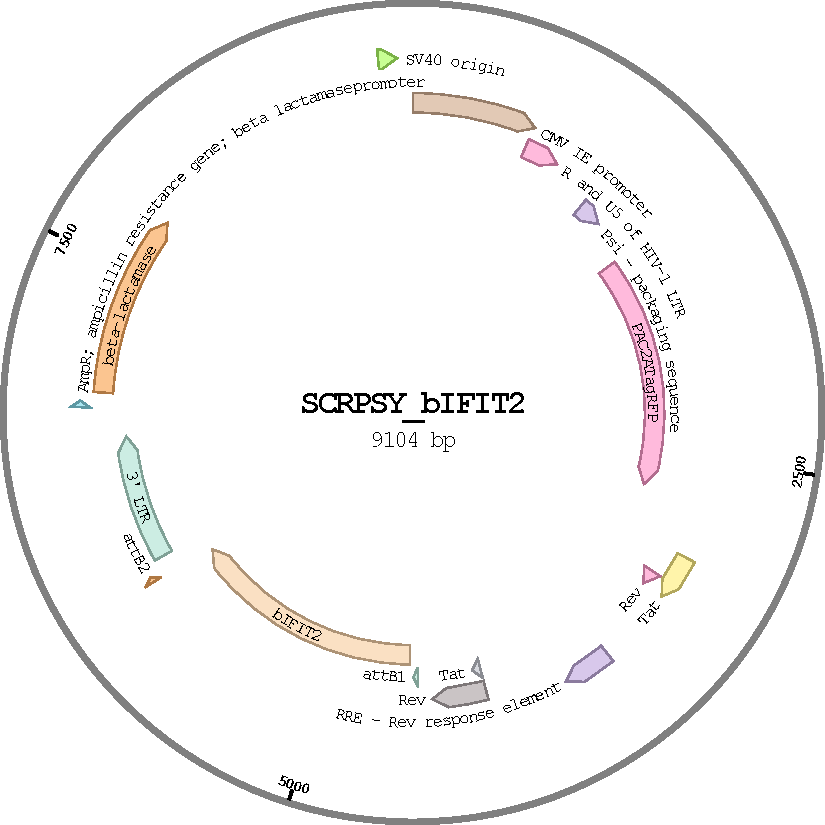
\includegraphics[width=0.6\linewidth]{05. Methods/Figs/scrpsy.pdf}
    \caption[SCRPSY Representative Map.]{\textbf{SCRPSY Representative Map.}}
    \label{fig:SCRPSY Representative Map}
\end{figure}

\begin{figure}
    \centering
    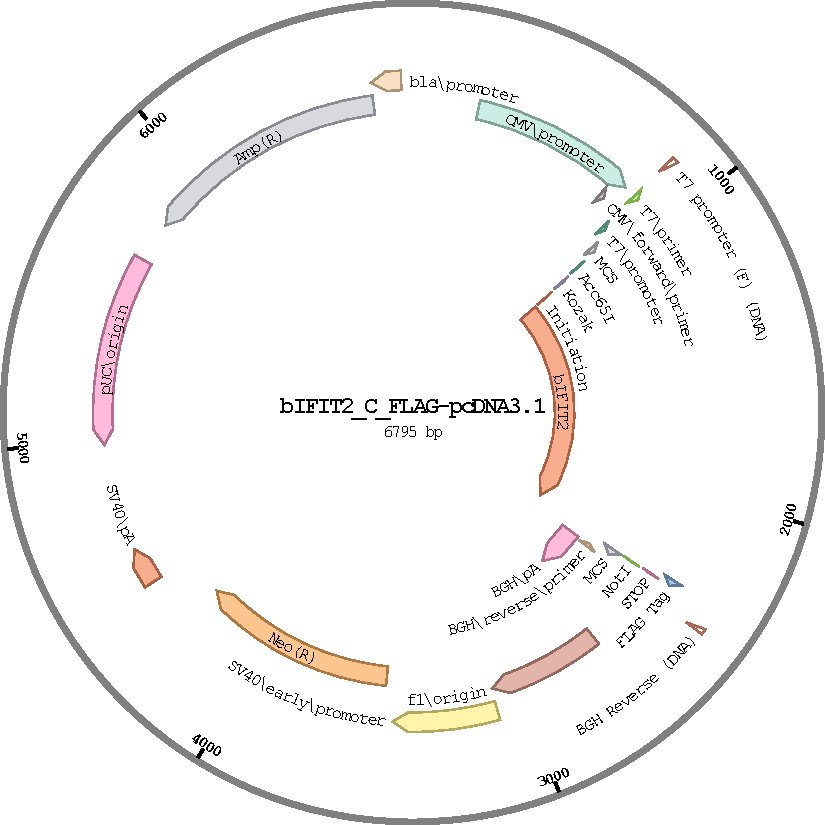
\includegraphics[width=0.6\linewidth]{05. Methods//Figs/pcDNA3.1.pdf}
    \caption[pcDNA3.1 Representative Map.]{\textbf{pcDNA3.1 Representative Map.}}
    \label{fig:pcDNA3.1 Representative Map}
\end{figure}




\subsection{Common Subcloning Methodologies} \label{subsec:Common Subcloning Methodologies}
\subsubsection[DNA Agarose Gel Electrophoresis and Extractions]{Analysis of DNA by Agarose Gel Electrophoresis and Gel Extractions} \label{Analysis of DNA by Agarose Gel Electrophoresis and Gel Extractions}
Linearised DNA was resolved and potentially isolated on 0.8\% agarose in Tris-Borate EDTA (TBE) buffer gel. 0.8\% agarose mixture was used as it provides resolution power greater than 10kbp-0.1kbp. DNA visualisation was enabled by the addition of 15 \(\mu\)L ethidium bromide into 50 mL agarose TBE solution at \~50°C prior to gel casting. DNA samples were mixed with 6X loading buffer (NEB) and loaded onto the gel. A DNA ladder was also electrophoresed in a separate well to allow size comparison. Samples were run at 80V for 90 minutes. After the run DNA bands were visualised using UV. Samples intended for gel purifications were excised from the gel using a clean scalpel and were placed into clean 1.5 mL tubes.




\subsubsection{DNA Clean-Up After PCR or Gel Extraction} \label{DNA Clean-Up After PCR or Gel Extraction}
DNA clean-up was performed using QiaQuick Gel Extraction kit (Quiagen) with accordance to the manufacturers protocol. In short, 3 volumes of buffer QC were added to either post PCR DNA or to a gel slice (where 1 mg of gel was assumed to be equivalent to 1 \(\mu\)L). Samples were incubated at 50°C for 10 minutes, after which one sample volume of isopropanol was added to the samples. Samples were collected on a QIAquick spin column via centrifugation and washed with buffer PE twice. DNA was eluted to 1.5 mL tube using centrifugation.




\subsubsection{DNA Ligation} \label{DNA Ligation}
20 \(\mu\)L total volume ligation reaction was prepared using DNA to be ligated, 2 \(\mu\)L T4 DNA ligase buffer (NEB) and 1 \(\mu\)L of T4 DNA ligase (NEB). Samples were incubated at 16°C for 72 hours.




\subsubsection[Transformation of \textit{E.Coli} and Bacterial Culture]{Transformation of Chemically Competent \textit{E.Coli} Cells and Bacterial Culture Amplification} \label{Transformation of Chemically Competent E.Coli Cells and Bacterial Culture Amplification}
2 \(\mu\)L of ligated samples or 1 \(\mu\)L of concentrated DNA were mixed with 25 \(\mu\)L \textit{E. coli} in 0.5 mL PCR tubes and were placed in a PCR cycler. Samples were initially incubated at 4°C for 15 minutes, following by heat shock performed by incubation at 42°C for 45 seconds followed by 2 minutes at 4°C. Afterwards, 75 \(\mu\)L of SOC solution was added and samples were left to incubate at 37°C for 60 minutes. Finally, 100 \(\mu\)L of transformed bacterial culture was streaked on room temperature agar plate containing ampicillin with a quadrant streaking method to ensure dilution gradient establishment on the plate allowing for single colony formation in the final quadrant. Plates were left to incubate for 24 hours at 37°C. Afterwards, single colonies were picked, annotated, and amplified in LB broth containing 1 \(\mu\)L per mL of ampicillin for 24 hours at 37°C.




\subsubsection{DNA Purification and Sequencing} \label{DNA Purification and Sequencing}
Bacterial cultures from the final step of Section \ref{Transformation of Chemically Competent E.Coli Cells and Bacterial Culture Amplification} were pelleted by centrifugation at 4°C for 30 minutes at 4000 g. Based on the size of the culture, the plasmid DNA was purified either by Miniprep or Midiprep kit (Quiagen; from 5 mL and 50 mL cultures respectively) based on the manufacturers protocol using the alkaline lysis method. Final purified DNA was quality assessed by restriction digestion followed by agarose gel electrophoresis (described in Section \ref{Analysis of DNA by Agarose Gel Electrophoresis and Gel Extractions}), which, if successful, was followed by sanger sequencing. Sequencing primers used to sequence ORFs of pcDNA3.1 plasmids were the forward T7 promoter primer and reverse BGH primer.




\subsection{PCR for Cloning into pcDNA3.1} \label{subsec:PCR for Cloning into pcDNA3.1}
In order to create tagged bovine \textit{IFIT} ORFs and subclone them from SCRPSY backbone into pcDNA3.1 backbone the following protocol was used. Primers were designed based on the schematic in \ref{fig:Schematic for PCR Primer Design}. The primers were 27-60 nucleotides in length. Their melting temperatures were established and used in the PCR protocol. PCR reaction mixtures with final volume of 100 \(\mu\)L were created by combining 10 \(\mu\)L of 10X Pfu Buffer (Promega) with 100 ng of plasmid DNA, 4 \(\mu\)L of 5 nM dNTPs (NEB), 2 \(\mu\)L of Pfu DNA polymerase (Promega), 1 \(\mu\)L of 100 \(\mu\)M forward and reverse primer and nuclease-free water. Samples were placed in PCR thermocycler and incubated for 30 seconds at 98°C. Followed were 30 cycles of 10 seconds at 98°C, followed by 30 seconds at 58°C and 90 seconds at 72°C. Final step was incubation at 72°C for 2 minutes. To degrade the original plasmid material, samples were incubated with DpnI restriction enzyme for 1 hour at 37°C. Afterwards, samples were cleaned as described in Section \ref{DNA Clean-Up After PCR or Gel Extraction}. The ORF amplicons had their ends digested by a sequential restriction digest with Acc65I (NEB) and NotI (NEB) restriction enzymes. This was done by diluting samples with 10X 3.1 buffer into 1X, adding restriction enzyme, incubation for 1 hour at 37°C and heat inactivation of enzyme at 65°C for 15 minutes. Digested amplicons were cleaned-up as described in Section \ref{DNA Clean-Up After PCR or Gel Extraction}. Donor plasmid pcDNA3.1 was linearised using Acc65I and NotI restriction enzymes as described above, and gel extracted as detailed in Section \ref{Analysis of DNA by Agarose Gel Electrophoresis and Gel Extractions} and \ref{DNA Clean-Up After PCR or Gel Extraction}. Linearised plasmid was dephosphorylated using Antarctic phosphatase (NEB). Amplicons and dephosphorylated plasmid were ligated in 5:1 molar ratio as described in Secton \ref{DNA Ligation}.

\begin{figure}
    \centering
    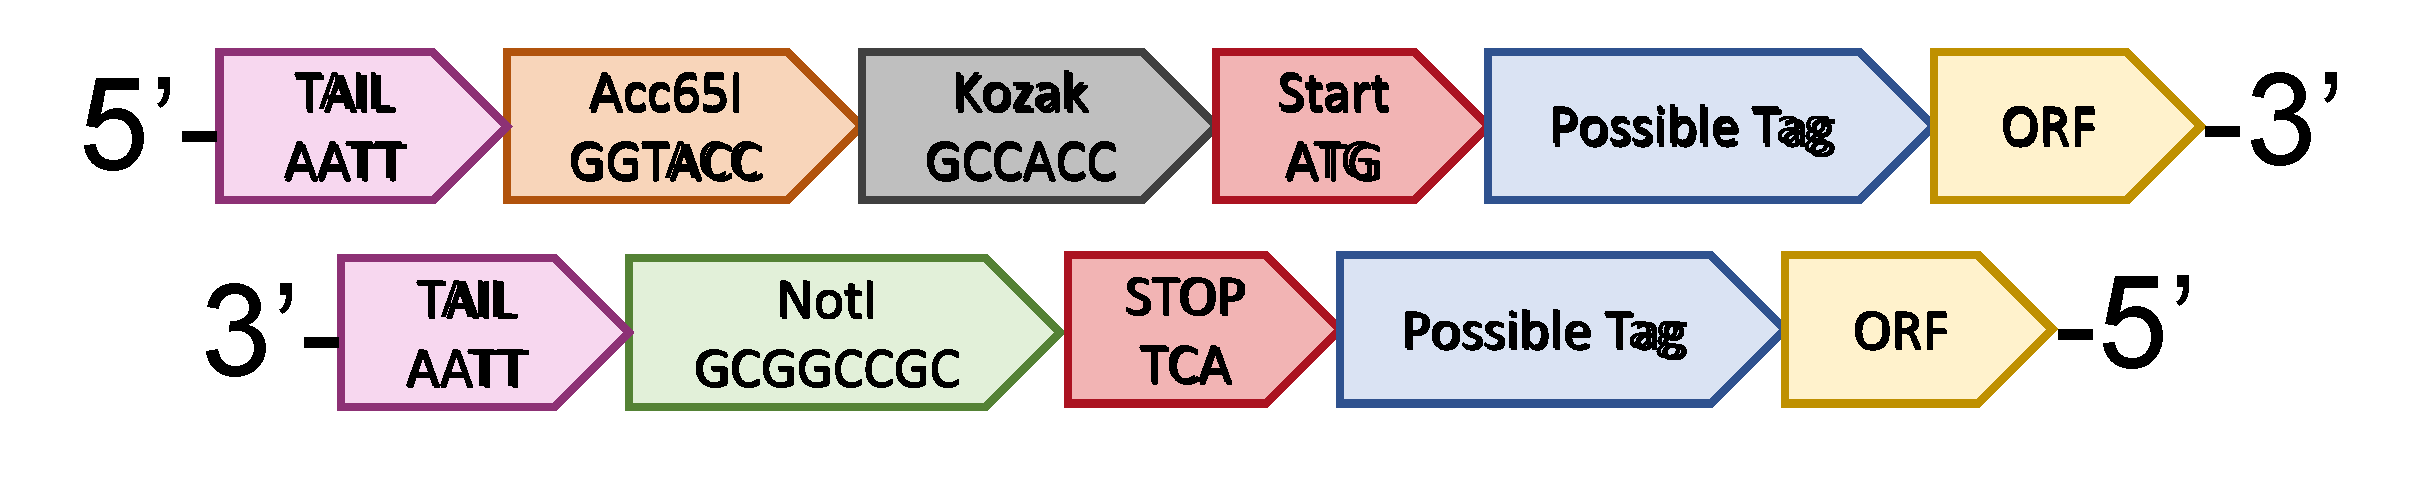
\includegraphics[width=1\linewidth]{05. Methods//Figs/cloning scheme.pdf}
    \caption[Schematic for PCR Primer Design.]{\textbf{Schematic for PCR Primer Design.}}
    \label{fig:Schematic for PCR Primer Design}
\end{figure}




\subsection{PCR for Point Mutant Generation} \label{subsec:PCR for Point Mutant Generation}
To create \textit{IFIT2} RNA-binding mutants a following protocol was used. Based on the publication in Tran \textit{et al.,} inverse PCR methodology was used with the primers for hIFIT mutations being taken from the study (\cite{Tran2020InfluenzaMRNAs}). bIFIT2 primers were based on the human ones. A protein model of human IFIT2 complex, visualised in PyMol software (\cite{SchrodingerTeam2023TheSystem}), had the amino acid residues 292 and 410 highlighted and compared to the residues on the corresponding place of predicted bovine IFIT2 structure. The effects of the mutations on the surfaces polarity assayed \textit{in silico}. This established that the corresponding amino acid residues on the bovine IFIT2 needed to be mutated were 287 and 401. The final primers can be seen in table Table \ref{tab:Primers for Inverse PCR Mutagenesis table}, where the mutating nucleotides are shown using lower case characters.
PCR reaction mixtures with final volume of 100 \(\mu\)L were created by combining 10 \(\mu\)L of 10X Pfu Buffer (Promega) with 100 ng of plasmid DNA, 4 \(\mu\)L of 5 nM dNTPs (NEB), 2 \(\mu\)L of Pfu DNA polymerase (Promega), 1 \(\mu\)L of 100 \(\mu\)M forward and reverse primer and nuclease-free water. Samples were placed in PCR thermocycler and incubated for 30 seconds at 98°C. Followed were 30 cycles of 10 seconds at 98°C, followed by 30 seconds at 58°C and 200 seconds at 72°C. Final step was incubation at 72°C for 2 minutes. To degrade the original plasmid material, samples were incubated with DpnI restriction enzyme for 1 hour at 37°C. Afterwards, samples were cleaned as described in Section \ref{DNA Clean-Up After PCR or Gel Extraction} and eluted in 20 \(\mu\)L of nuclease-free water. DNA was phosphorylated by adding 2\(\mu\)L of 10X ligase buffer and 1 \(\mu\)L of T4 Polynucleotide Kinase (NEB) and incubating the samples for 30 minutes at 37°C. The enzyme was inactivated by incubation at 65°C for 20 minutes. Samples were then ligated by addition of 1 \(\mu\)L of T4 DNA ligase and incubation at 16°C for 72 hours.

\begin{table}
\centering
\begin{tabular}{ll}
\hline
\textbf{Primer Name}   & \textbf{Sequence 5'-3'}    \\ \hline
hIFIT2   R292E forward & GTGCTGCTATgagGCAAAAGTCTTC  \\ \hline
hIFIT2 R292E reverse   & CCAATTTGGCAATGCAGG         \\ \hline
hIFIT2   K410E forward & GGAGAAAGAAgagATGAAAGACAAAC \\ \hline
hIFIT2 K410E reverse   & CTTGATTTCTGGTTTATTTTTACAC  \\ \hline
bIFIT2   R287E forward & GTGCTGCTATgagGCCAAAGTCCT   \\ \hline
bIFIT2 R287E reverse   & CCAATATGGCAATGCAGG         \\ \hline
bIFIT2   K401E forward & GAAGGAGAAgaaATGAAAAACAAAC  \\ \hline
bIFIT2 K401E reverse   & CTTTGATCCCTGGTTTAT         \\ \hline
\end{tabular}
\caption[Primers for Inverse PCR Mutagenesis.]{\textbf{Primers for Inverse PCR Mutagenesis.}}
\label{tab:Primers for Inverse PCR Mutagenesis table}
\end{table}




\section{Protein Work} \label{sec:Protein Work}
\subsection{Immunoprecipitation} \label{subsec:Immunoprecipitation}
Immunoprecipitation (IP) and co-immunoprecipitation (co-IP) was performed to isolate specific proteins or protein complexes, respectively. 2,000,000 HEK293T cells were seeded in a 10 cm dish. For transfection experiments 7.7 \(\mu\)g of DNA was transfected as described in Section \ref{subsec:Transfecting Cells}. 24 hours post transfection cells, or at the terminal point of experiment cells were scraped and transferred into a 50 mL conical tube. Cells were repeatedly spun down and washed with PBS until there was no residual contamination from culture media. Final cell pellet was resuspended in 1 mL of cold lysis buffer (10 mM Tris/HCl pH 7.5; 150 mM NaCl; 0.5 mM EDTA; 0.5\% NP-40; 1:100 protease inhibitors (Sigma)) and incubated for 30 minutes on ice. Afterwards samples were spun down at 20,000 g for 10 min at 4°C and the supernatant was transferred into pre-cooled tube. Dynabead protein-G beads (ThermoFisher) were bind to a target antibody by combining 50 \(\mu\)L of magnetic beads with 5 \(\mu\)g of target antibody in 200 \(\mu\)L of PBS with Tween 20 for 10 minutes at room temperature. Afterwards, using a magnet, the supernatant was removed without removing the bead-antibody complexes. After the beads were resuspended in lysis buffer. After centrifuging the lysates were added to the beads and incubated using a rotor for 30 minutes at 4°C. Afterwards the samples were washed twice using magnetic rack and a wash buffer (10 mM Tris/HCl pH 7.5; 150 mM NaCl; 0.5 mM EDTA). After the final wash was removed the bead-sample complexes were resuspended in 45 \(\mu\)L 2x SDS loading buffer, incubated at 95°C for 5 minutes. Afterwards the samples were centrifuged at top speed for 2 minutes and the pellet was discarded. This was the \textbf{bound} sample, which contained the immunoprecipitated target, along with the antibody which was used to precipitate it. During the experiment two additional samples were aliquoted, each 50 \(\mu\)L in volume. First was after centrifugation of the lysates (\textbf{input} sample) and the second after incubation of lysates with the beads on rotor (\textbf{unbound} sample). Both of these samples were mixed 1:1 with 2x SDS loading buffer and boiled at 95°C for 5 minutes.




\subsection{SDS-PAGE and Western Blotting} \label{subsec:SDS-PAGE and Western Blotting}
At the end point of experiments with cells, the growth medium was removed, and the cells were washed with PBS. Cells were lysed in 1X Laemmli SDS sample buffer (Bio-Rad) supplemented with \(\beta\)-mercaptoethanol (Sigma) and denatured by boiling at 95°C for 5 minutes. Samples were run on 10\% SDS polyacrylamide gels. The running gel was prepared using 10-\% v/v polyacrylamide (Protogel), 0.39 M Tris pH 8.8, 0.1\% w/v SDS, 0.1\% w/v ammonium persulphate (APS) and 0.04\% w/v tetramethylethylenediamine (TEMED; Bio-Rad). The stacking gel consisted of 5\% v/v polyacrylamide, 0.13 M Tris pH 6.8, 0.1\% w/v SDS, 0.1\% w/v APS and 0.1\% w/v TEMED. PageRuler Plus prestained protein ladder (Thermo Scientific) was used as a molecular weight marker. Samples were run in a Mini-PROTEAN Tetra Vertical Electrophoresis Cell (BioRad) at 110 V for 120 minutes. Afterwards the proteins were transferred into polyvinylidene difluoride (PVDF) membranes (Bio-Rad) using the Trans-blot Turbo blotting system (Bio-Rad) with 1X transfer buffer (25 mM Tris, 192 mM glycine, pH 8.3; Bio-Rad) following the manufacturer’s instructions (30 min at 25 V). Afterwards the membranes were blocked by incubation with with 5\% (w/v) skimmed milk in PBS with 0.1\% Tween 20 (PBST) for an hour. Afterwards the membranes were washed several times with in PBS with 0.1\% Tween 20. During this step it is possible to reversible visualise proteins on the membrane using Ponceau S (ThermoFisher). After washing steps the membranes were incubated with milk-PBST-primary antibody mixtures overnight at 4°C, washed three times with PBS-T and probed with either horseradish peroxidase-conjugated secondary antibodies or fluorophore-conjugated secondary antibodies, diluted in 5\% milk in PBST. Protein bands were detected either directly or using Clarity Western ECL substrate (Bio-Rad) and imaged with Bio-Rad ChemiDoc MP Imaging System.




\section{Confocal Microscopy} \label{sec:Confocal Microscopy}
Cells grown on a glass coverslip with 13 mm diameter (Agar Scientific) were washed with PBS and fixed by incubating for 15 minutes with room temperature 4\% paraformaldehyde (Sigma-Aldrich) at the end point of the experiments. Samples were subsequently permeabilised by being incubated in 0.2\% Triton X-100/PBS solution for 5 minutes. Residual Triton was removed by PBS washes, after which the coverslips were blocked using 1\% bovine serum albumin (BSA; Sigma-Aldrich) in PBS for at least 30 minutes. Samples were then incubated overnight with the primary antibody 1\% BSA in PBS solution, diluted as specified in Table \ref{tab:Antibodies for Confocal Microscopy}. Afterwards, they were washed again with PBS and incubated for an hour at room temperature with secondary antibodies diluted in 1\% BSA in PBS solution, as specified in Table \ref{tab:Antibodies for Confocal Microscopy}. Nuclei of the cells were stained by 4,6-diamidino-2-phenylindole (DAPI; Abcam), diluted 1:20,000 in water. After 10-minute incubation, residual DAPI was washed away by water, following by an additional was with PBS. Stained slides were mounted on glass slides using Vectashield (Vector Labs). Confocal images were acquired on Leica TCS SP5 and Zeiss LMS700 confocal microscopes using 405 nm, 488 nm, and 568 nm laser lines with 63X oil immersion objective. Laser lines were operated in sequential manner to prevent bleed-through and the image quality was enhanced by frame averaging. The pinhole was set to 1 airy unit. Maximal laser line gains were established per experiment using secondary antibody only controls, while minimal gains were established using the maximum intensity of sample slides, allowing for maximum range of signal acquisition. Image analysis was conducted in FiJi (\cite{Schindelin2012Fiji:Analysis}) and final figures were constructed using QuickFigures FiJi plugin (\cite{Mazo2021QuickFigures:Figures}).


\begin{table}
\centering
\begin{tabular}{@{}cccc@{}}
\toprule
\textbf{Antibody Target} & \textbf{Host Species} & \textbf{Provider} & \textbf{Working Dilution} \\ \midrule
RSV N       & Mouse  & Abcam             & 1:400   \\
RSV P       & Mouse  & FILL              & 1:400   \\
RSV   M2/1  & Mouse  & FILL              & 1:400   \\
IFIT1       & Rabbit & Invitrogen        & 1:200   \\
IFIT2   (A) & Rabbit & Proteintech       & 1:200   \\
IFIT2 (B)   & Rabbit & Novus Biologicals & 1:200   \\
IFIT3       & Rabbit & Proteintech       & 1:200   \\
IFIT5       & Rabbit & Invitrogen              & 1:200   \\
FLAG        & Rabbit & Invitrogen              & 1:200   \\
Rabbit Igg  & FILL   & Invitrogen              & 1:10000 \\
Mouse   Igg & FILL   & Invitrogen              & 1:10000 \\ \bottomrule
\end{tabular}
\caption[Antibodies for Confocal Microscopy.]{\textbf{Antibodies for Confocal Microscopy.}}
\label{tab:Antibodies for Confocal Microscopy}
\end{table}




\section{RNAseq Differential Expression Analysis} \label{sec:RNAseq Differential Expression Analysis}
RNAseq experiments comparing the transcript levels between control cells and cells infected with either wild-type bovine RSV or bovine RSV with a deleted SH gene, either 16 and 40 hours post infection were previously performed by Dr. Fouthemata Jobe from the Viral Glycoproteins Group at the Pirbright Institute. The initial data analysis was performed by the bioinformatics team of the Pirbright Institute. They included the viral genes as a part of the analysis and therefore these were the only differentially expressed genes from the study. I have reanalysed the counts dataset, which had viral genes omitted. Data processing, statistical analysis and graph generation was conducted R programming language (\cite{RCoreTeam2022R:Computing}) using RStudio enviroment (\cite{RStudioTeam2022RStudio:RStudio}). Initial exploratory data analysis and differential expression analysis was done using the DESeq2 R package (\cite{Love2014ModeratedDESeq2}). Viral genes were filtered from the dataset pre analysis. After creation of DESeq2 object, genes with no counts were filtered. To perform initial exploratory data analysis and visualization data was transformed using regularized logarithm (rlog) and the variance stabilizing transformation (VST) methods. This was done to stabilize the variance across the mean. The transformed data was visualised using the principal component analysis (PCA) plot and sample distance matrix. Following this the differential expression analysis was performed on non-transformed filtered data. Following the recommendation of Schurch \textit{et al.}, the fold-change threshold was set to 0.5 and the minimum adjusted p value was set to 1\% to optimise the true positive rate and false positive rates (\cite{Schurch2016HowUse}). The data was visualised by volcano plots, MA plots and heatmaps (using pheatmap R package (\cite{Kolde2019Pheatmap:Heatmaps})). The final dataset was annotated with the appropriate gene names and gene symbols from latest available bovine genomic dataset using org.Bt.eg.db R package (\cite{Carlson2022Org.Bt.eg.db:Bovine}).




\section{Statistical Analysis} \label{sec:Statistical Analysis}
Statistical analysis was performed using R programming language (\cite{RCoreTeam2022R:Computing}) using the RStudio environment (\cite{RStudioTeam2022RStudio:RStudio}). The pipeline can be viewed in the following URL: http://rpubs.com/ogosimiso/995988. Initially, data was assessed visually using boxplots and Q-Q plots. Boxplots were used to roughly assess the normality, whereas Q-Q plots were used for rough equality of variance assumptions. A mathematical test of the normality of distribution was done using the Shapiro-Wilk normality test. This was performed on each individual condition as well as the whole dataset in its entirety. Mathematical assessment of equality of variance was done by Bartlett test of homogeneity of variances for normally distributed samples and by Levene's Test for Homogeneity of Variance (car package for R (\cite{Fox2019AnRegression})) for non-normally distributed samples. To obtain the final significance values various mathematical tests were used based on the number of comparisons and the previously established type of distribution and equality of variance. For a pair of samples with normal distribution and equal variance a two-sample t-test was conducted. For multiple comparisons of normally distributed data with equal variance analysis of variance (ANOVA) combined with Tukey multiple comparison of means was performed. For a pair of samples with non-normal distribution but equal variance, a two-sample t-test was conducted. For multiple comparisons of non-normally distributed data with equal variance a Kruskal-Wallis rank sum test was performed (dunn.test R package (\cite{Dinno2017Dunn.test:Sums})). For a single comparison of data which has normal distribution but non-equal variance a Welch Two Sample t-test was performed. For multiple comparisons of data with normal distribution but non-equal variance one-way analysis of means (not assuming equal variances) combined with Games-Howell test was performed (rstatix R package (\cite{Kassambara2022Rstatix:Tests})). 

%acronyms
\nomenclature[z-DMEM]{$DMEM$}{Dulbecco’s Modified Eagle’s Medium} 
\nomenclature[z-FBS]{$FBS$}{Foetal Bovine Serum }    
\nomenclature[z-PBS]{$PBS$}{Phosphate Buffered Saline}    
\nomenclature[z-IFN]{$IFN$}{Interferon}  
\nomenclature[z-ANOVA]{$ANOVA$}{Analysis of Variance} 
\nomenclature[z-PCA]{$PCA$}{Principal Component Analysis} 
\nomenclature[z-VST]{$VST$}{Variance Stabilizing Transformation} 
\nomenclature[z-rlog]{$rlog$}{Regularized Logarithm} 
\nomenclature[z-DAPI]{$DAPI$}{4,6-diamidino-2-phenylindole} 
\nomenclature[z-BSA]{$BSA$}{Bovine Serum Albumin} 
\nomenclature[z-PBST]{$PBST$}{PBS with 0.1\% Tween 20} 
\nomenclature[z-PVDF]{$PVDF$}{polyvinylidene difluoride} 
\nomenclature[z-TEMED]{$TEMED$}{tetramethylethylenediamine} 
\nomenclature[z-APS]{$APS$}{ammonium persulphate}  
\nomenclature[z-IP]{$IP$}{Immunoprecipitation}  
\nomenclature[z-co-IP]{$co-IP$}{co-immunoprecipitation}  
\nomenclature[z-TBE]{$TBE$}{Tris-Borate EDTA}  
\nomenclature[z-ORFs]{$ORFs$}{Open Reading Frames}  
\nomenclature[z-GFP]{$GFP$}{Green Fluorescent Protein}  
\nomenclature[z-MOI]{$MOI$}{Multiplicity of Infection}  
\nomenclature[z-PEG]{$PEG$}{Polyethylene Glycol}  
\nomenclature[z-cDNA]{$cDNA$}{Complementary DNA}  
\nomenclature[z-qPCR]{$qPCR$}{Quantitative Polymerase Chain Reaction}  
\nomenclature[z-Ct]{$Ct$}{Cycle Threshold}  
\nomenclature[z-MMLV RT]{$MMLV RT$}{Moloney Murine Leukaemia Virus Reverse Transcriptase}  